\chapter{Marco Teórico}

El proyecto es un sistema interactivo que busca proporcionar al usuario independientemente de sus intereses, el cumplimiento de sus expectativas, siendo un desarrollo a conciencia, pero sin tomarlo demasiado en serio, busca también romper el estereotipo que imponen los proyectos de esta modalidad, que si bien, ofrecen un producto de relativa buena calidad y mantenimiento, son o bien productos comerciales como es el caso de Just Dance o productos privatizados como son los desarrollados para la medicina. 

En cambio, se tiene la expectativa de ofrecer al nivel de Open source del proyecto, que a la larga atraiga a más miembros, al igual que Linux o Apache y pueda expandir sus horizontes y calidad del producto, teniendo presente que Open Source no significa simplemente compartir el acceso al código fuente, como indica la \href{https://opensource.org/docs/definition.html}{Open Source Definition (OSD)}. 

El desarrollo del proyecto empleara los recursos disponibles y al alcance de cualquier desarrollador, por tanto, no tomara en cuenta el manejo de cámaras de profundidad, esta aclaración es necesaria, ya que la calidad del producto final puede ser muy variable al de proyectos similares y es una característica más por la que sobresaldría este proyecto, ya que reduciría el presupuesto necesario para el consumidor.\\

A continuación, se debe mencionar factores importantes sobre la implementación del proyecto, como las propiedades del Body Tracking, la verdadera forma que tiene esta herramienta que tiene para ofrecer al software, por que no sobra mencionar las distinciones entre una cámara normal y una de profundidad, así como un breve vistazo a la legalidad que sigue rígidamente el proyecto.

\section{Body Tracking/Motion Capture}

El seguimiento corporal del cuerpo, normalmente conocido como Body Tracking o Motion Capture hace referencia al seguimiento del cuerpo humano a través de una cámara, existen dos acercamientos a este estudio, el enfoque de ajuste del modelo y el enfoque de aprendizaje. El enfoque de ajuste del modelo involucra ajustar el modelo formulado según imágenes previas cargadas, estimando parámetros de puntos especificados de la imagen, sin embargo, es demasiado dependiente de extremos locales y la inicialización adecuada, lo cual lo vuelve inservible en ambientes nuevos. Este modelo comparte una similitud al método Monte Carlo basados en cadenas de Markov \cite{siddiqui2010human}.

En cambio, el enfoque de aprendizaje requiere de grandes cantidades de imagenes con notas y especificaciones del esqueleto en las imagenes, incrementando las dimensiones de espacio y memoria requerido. Un ejemplo de este tipo de reconocimiento es la herramienta PoseNet, derivado de TensorFlow, empleado para identificar objetos a partir de una base de datos propia que clasifique los elementos que se buscan identificar con silueta y nombre.

\begin{figure}[t!]
	\centering
	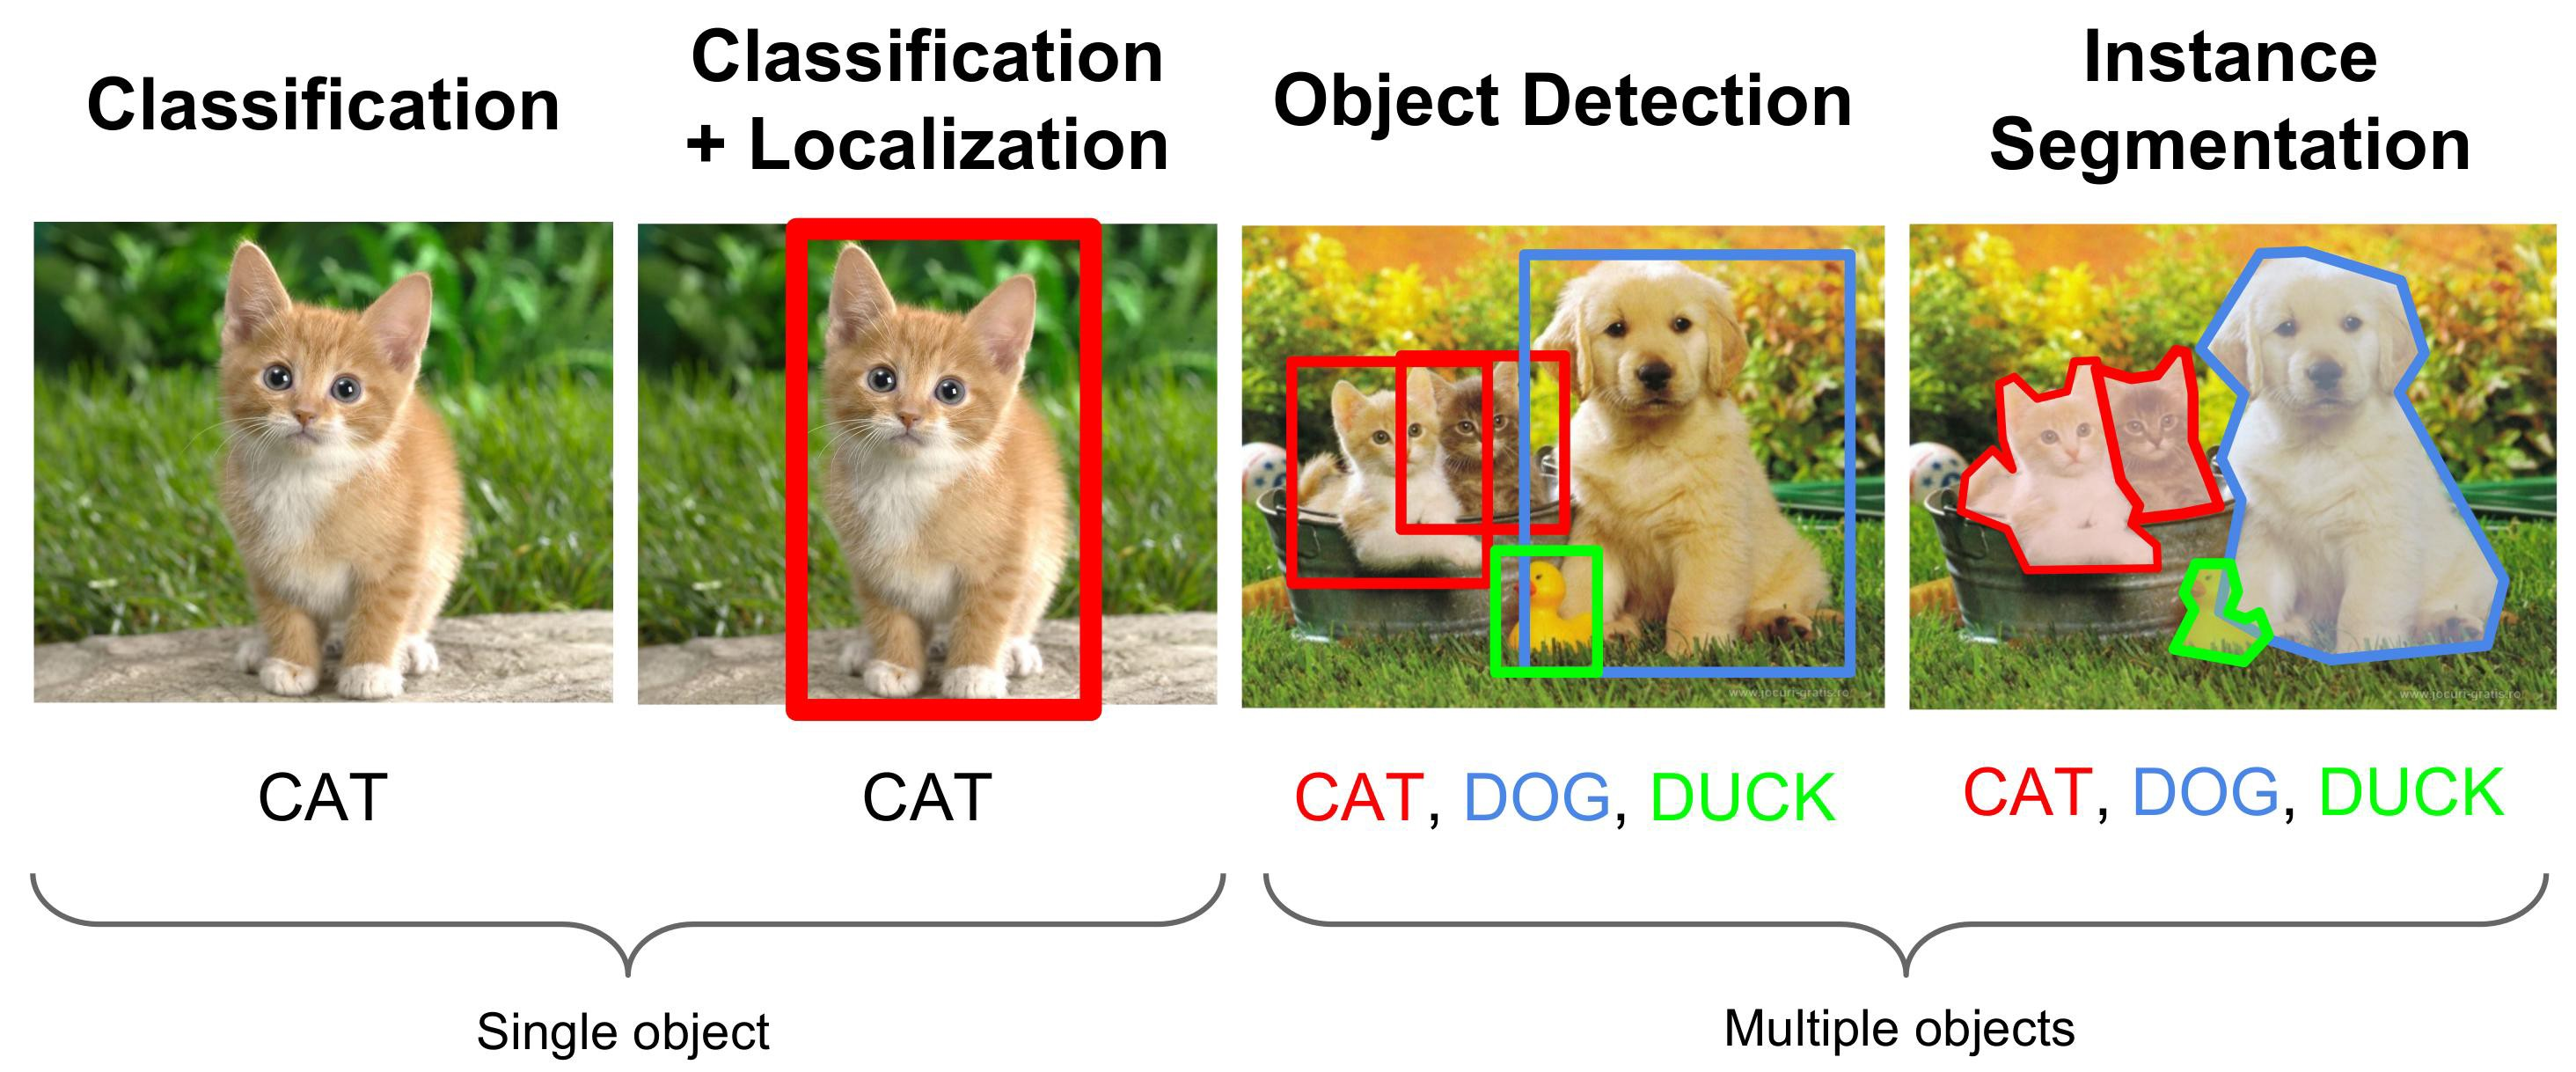
\includegraphics[width=13cm,height=5cm,]{./Images/ejemplotensorflow.jpg}
	\caption{Ejemplo de Clasificación de imagen de TensorFlow}
	\label{tensorfl}
\end{figure}

Finalmente se empleo la iteración del punto más cercano \cite{grest2005nonlinear} el cual usa un enfoque de inicialización del esqueleto a través de fotogramas subsecuentes, clasificándolos con vértices y segmentos en un modelo 3D para este propósito.

La estimación de las poses humanas representan una problemática compleja de solucionar, el cual tuvo un largo trayecto hasta salir a la luz. La complejidad se centra en las múltiples limitantes, como las mascotas, los objetos del área, las personas de alrededor, la variación del escenario, los parámetros del cuerpo (el tamaño, longitud de las extremidades, torso y otras partes del cuerpo) y la iluminación.

Empleando las herramientas de seguimiento del Esqueleto, sensores de profundidad y sensores RGB, a medida que el tiempo corre, la necesidad de herramientas como los sensores va volviéndose obsoleta con el nacer de herramientas como PoseNet y OpenPose, que con el apoyo del Hardware mínimo necesario, son capaces de proporcionar la misma calidad de seguimiento corporal.


\subsection{Skeletical Tracking}

Este fue una innovación brindada por el controlador Kinect al mercado comercial, Su demanda fue elevada en la época y hasta el día de hoy sigue siendo empleado, el reconocimiento de una persona desde cualquier angulo o distancia, tomando en cuenta su figura, tamaño, colo, cabello, ropa y el ambiente. Se emplea el escaneo de la imagen para reconocer puntos importantes del cuerpo que representan al cuerpo, tales como la cabeza, cuello, hombros, brazos, piernas y otros 10 a 20 puntos dependiendo la herramienta de reconocimiento que se emplee.
\begin{figure}[ht]
	\centering
	\begin{subfigure}{.3\textwidth}
		\centering
		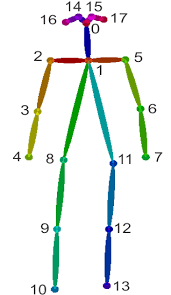
\includegraphics[width=3cm,height=4cm]{./Images/openposet1.png}
		\caption{Reconocimiento OpenPose Tipo BODY\_25}
		\label{open1}
	\end{subfigure}%
	\begin{subfigure}{.3\textwidth}
		\centering
		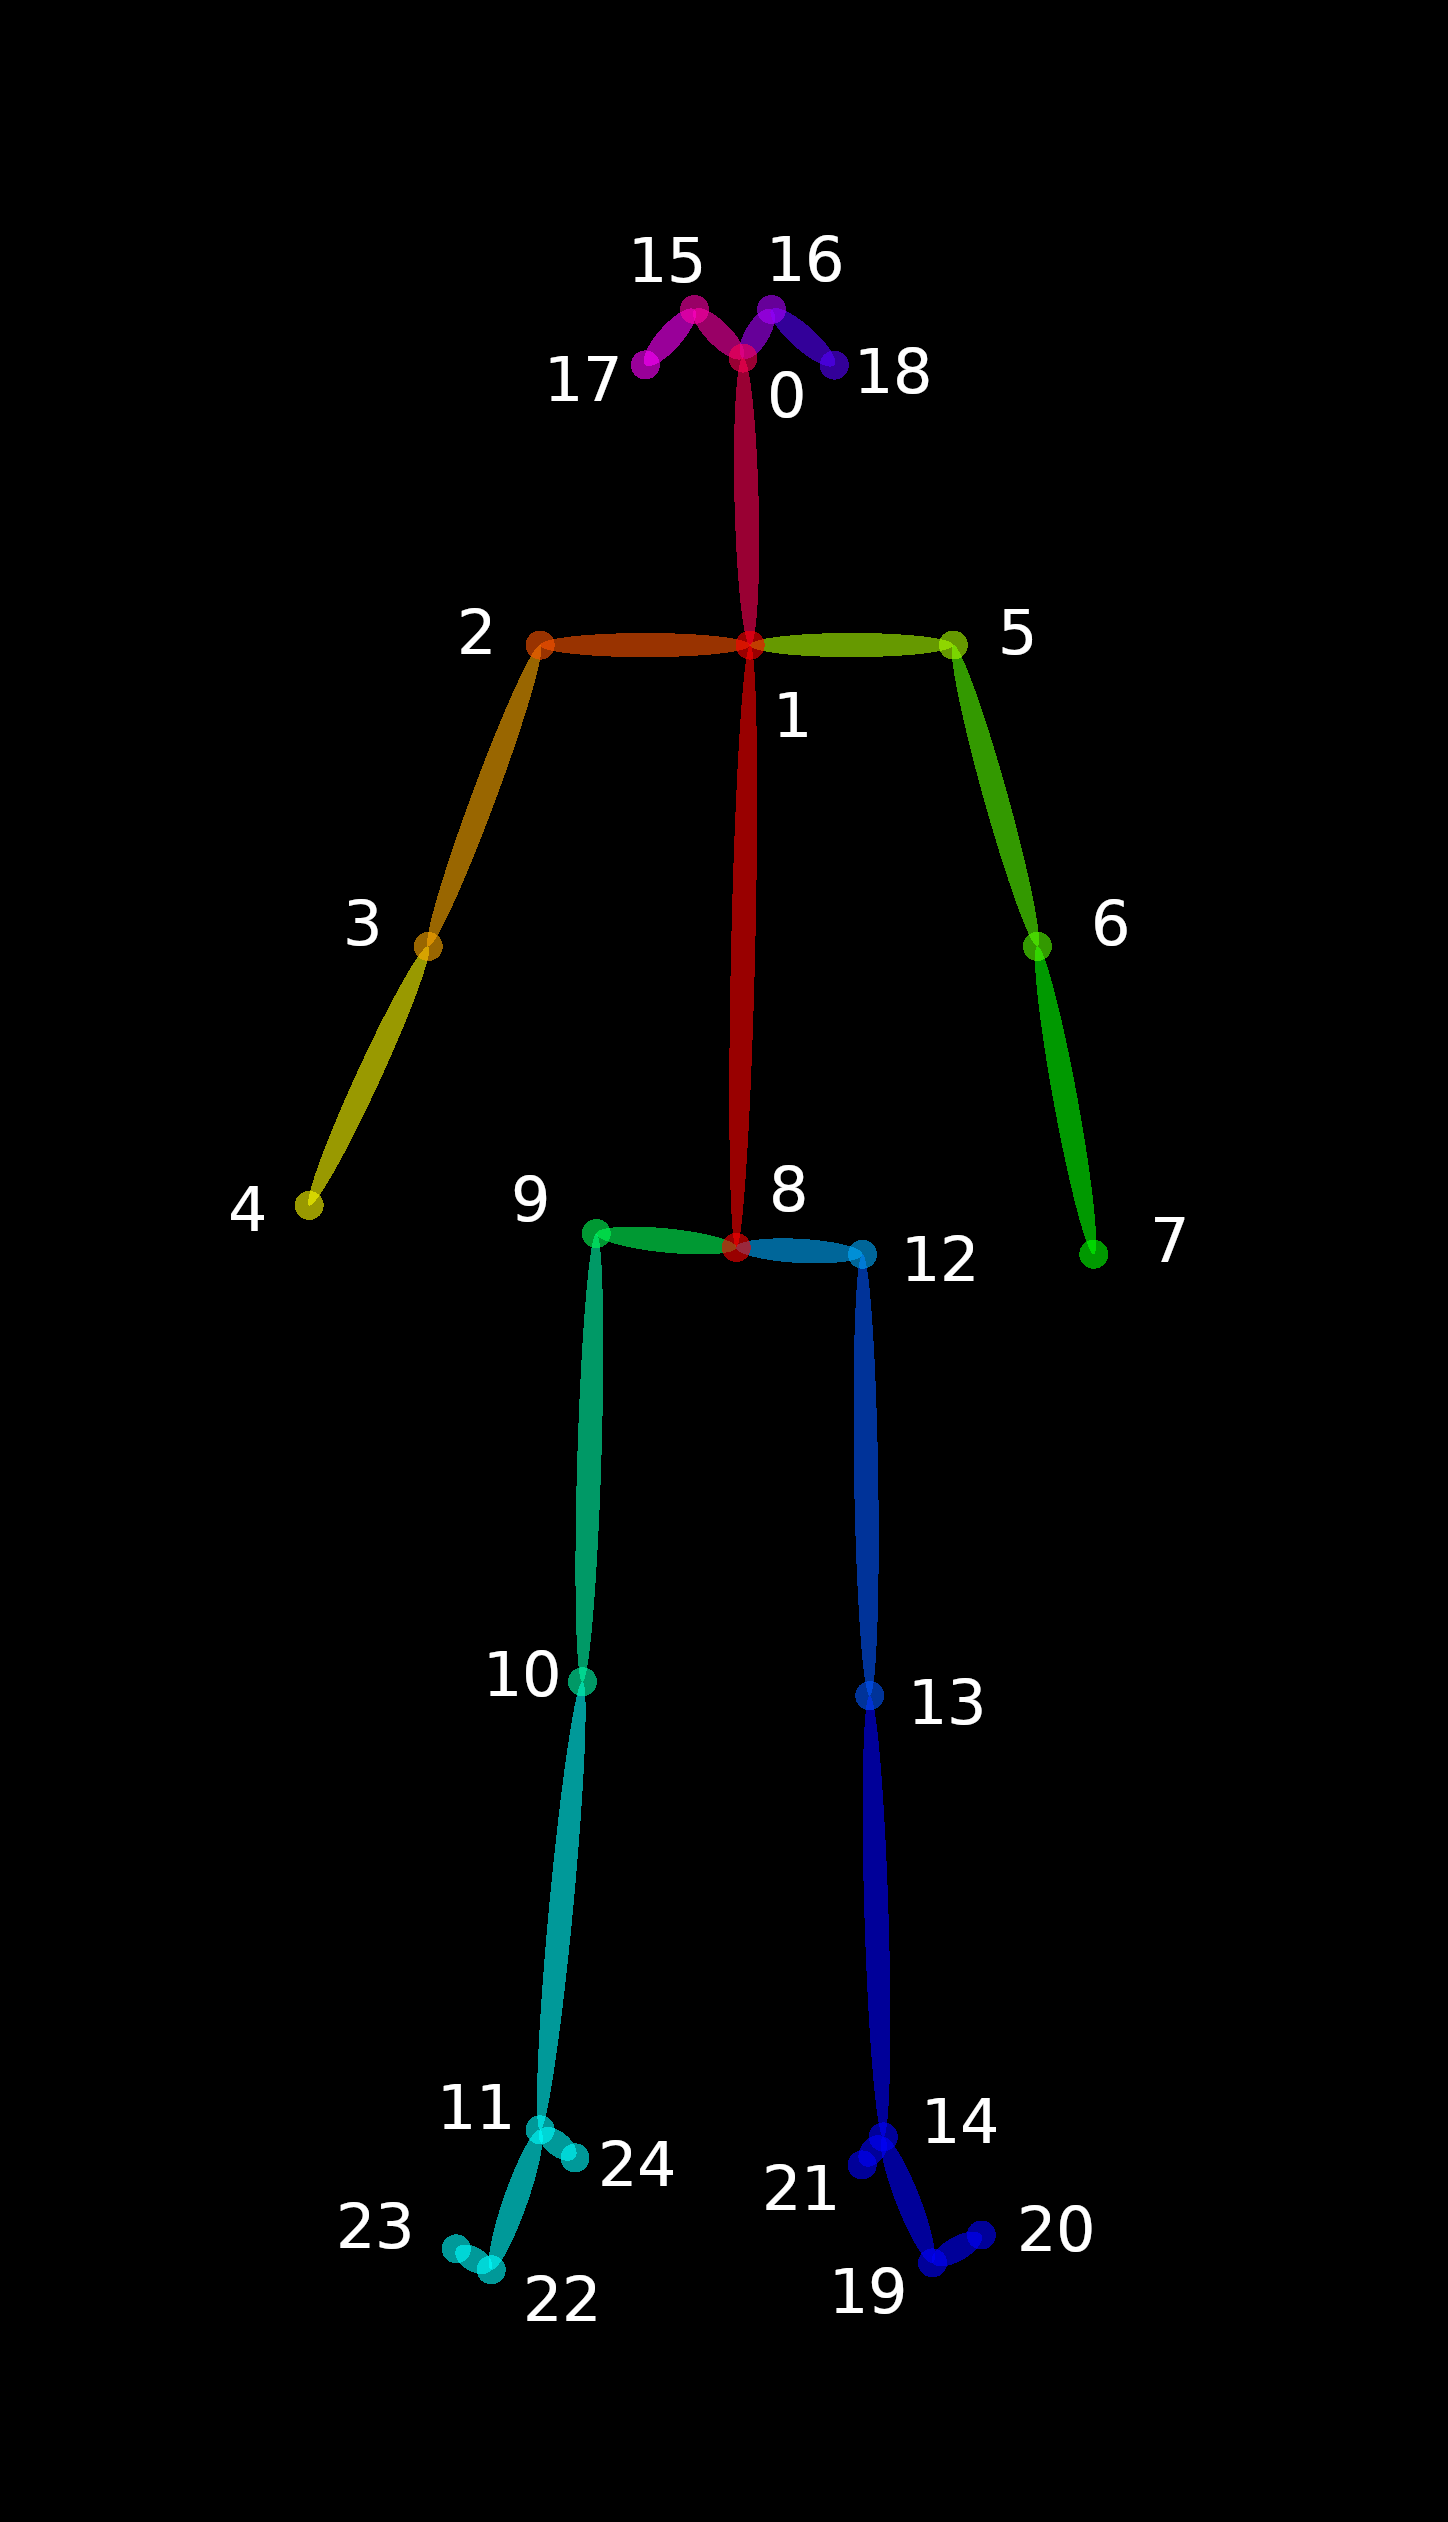
\includegraphics[width=3cm,height=4cm]{./Images/openposet2.png}
		\caption{Reconocimiento OpenPose Tipo COCO}
		\label{open2}
	\end{subfigure}%
	\begin{subfigure}{.3\textwidth}
		\centering
		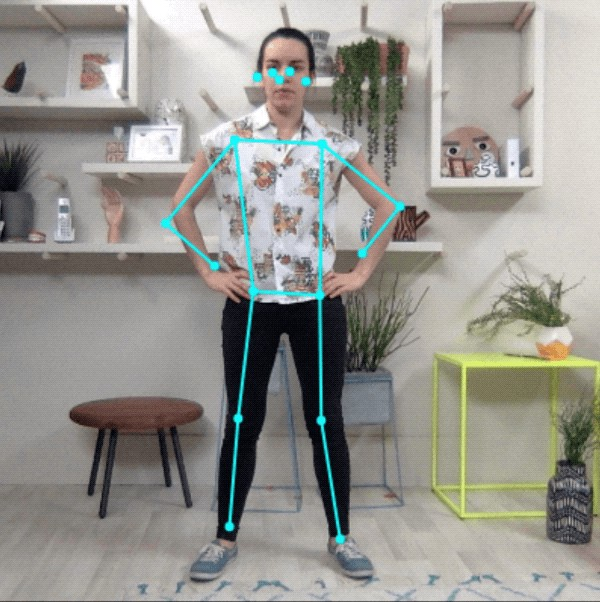
\includegraphics[width=3cm,height=4cm]{./Images/posenetexa.jpg}
		\caption{Reconocimiento PoseNet }
		\label{posenet1}
	\end{subfigure}
	\caption{Diversos Tipos de Seguimiento al Esqueleto}
	\label{exampleesqueletotrack}
\end{figure}

La herramienta seleccionada para el proyecto es OpenPose empleando este modelo de \href{https://github.com/CMU-Perceptual-Computing-Lab/openpose/blob/master/doc/output.md}{Formato de salida}, para los datos del seguimiento del esqueleto es emplear la flag write\_json para guardar la información dentro un JSON, el cual contiene un objeto de esqueleto de persona dentro, que contiene un vector pose\_keypoints\_2d con puntos 2D para localizar y detectar cada punto de unión x1,y1,c1,x2,y2,c2,.... Las coordenadas x y y en el rango de [0,1], [-1,1].

Además de la existencia de los vectores face\_keypoints\_2d, hand\_left\_keypoints\_2d y hand\_right\_keypoints\_2d, análogos a pose\_keypoints\_2d, los cuales debido a la masiva carga de memoria que requieren y la falta de ella (mínimo 4GB de Memoria dedicada estimada, contando solo con 2GB en el equipo proporcionado) serán ignorados, pero empleando pose\_keypoints\_2d.

Como dato, los vectores análogos body\_keypoints\_3d, face\_keypoints\_3d,
hand\_left\_keypoints\_2d y hand\_right\_keypoints\_2d (si --3d flag se habilitase), en vez de 
x1,y1,c1,x2,y2,c2,..., el formato sería x1,y1,z1,c1,x2,y2,z2,c2,..., donde 0 sería 1 o 0 dependiendo si la reconstrucción 3D es exitosa.

Se empleara el API de BODY\_25 para mostrar el esqueleto, que consiste en mostrar 25 puntos del esqueleto, cada uno con su conexión en los siguientes puntos clave:

\{0,  "Nose"\}, \{1,  "Neck"\}, \{2,  "RShoulder"\}, \{3,  "RElbow"\}, \{4,  "RWrist"\}, 
\{5,  "LShoulder"\}, \{6,  "LElbow"\}, \{7,  "LWrist"\}, \{8,  "MidHip"\}, \{9,  "RHip"\},
\{10, "RKnee"\}, \{11, "RAnkle"\}, \{12, "LHip"\}, \{13, "LKnee"\}, \{14, "LAnkle"\}, 
\{15, "REye"\}, \{16, "LEye"\}, \{17, "REar"\}, \{18, "LEar"\}, \{19, "LBigToe"\},
\{20, "LSmallToe"\}, \{21, "LHeel"\}, \{22, "RBigToe"\},\{23, "RSmallToe"\},\{24, "RHeel"\},
\{25, "Background"\}


En cuanto al resultado, este se puede guardar en formatos estándar (JSON, XML, PNG, JPG,...), existen suficientes herramientas de uso libre para leerlos, por tanto cargar los datos y cargar las imagenes, no debería representar un desafio.



\subsubsection{Normalización de Imagenes Empleando Dssim/TensorFlow}

En espera, todavía no hay nada para saber como comparar imagenes




